% add --shell-escape to pdflatex arguments.
% add following key to have keyboard shortcuts
%{
%    "key": "shift+b",
%    "command": "commandId",
%    "when": "editorTextFocus"
%},
%{
%"key": "shift+B",
%"command": "editor.action.insertSnippet",
%"when": "editorLangId == latex && editorTextFocus",
%"args": {
%    "snippet": "\\textbf{${TM_SELECTED_TEXT}$0}"
%}
%}

\documentclass[14pt]{extarticle}
\usepackage[left=0.5cm , right = 0.5cm, top=0.5cm]{geometry}
\usepackage{helvet}
\usepackage{parskip}
\usepackage{amsmath}
\usepackage{amssymb}
\usepackage{graphicx}
\usepackage[spanish]{babel}
\usepackage[dvipsnames]{xcolor}
\usepackage{tcolorbox} % above of the svg package
\usepackage{svg} 
\usepackage{hyperref}
\usepackage{minted}
\renewcommand{\sfdefault}{lmss}  % este activa la letra lmss
\renewcommand{\familydefault}{\sfdefault} % este activa la letra lmss
\sffamily % este activa la letra lmss
%\hyperlink{page.2}{Go to page 2}
%\newpage
%text on page 2
%\begin{figure}[htbp]
%  \centering
%  \includesvg{plot.svg}
%  \caption{svg image}
%\end{figure}

%\begin{minted}{csharp}
%    // single comment
%    \end{minted}

% f(n) = \begin{cases}
%    n/2  & n \text{ is even} \\
%    3n+1 & n \text{ is odd}
%  \end{cases}

%\begin{align}
%    \frac{d}{dx} \ln x &= \lim_{h\to 0} \frac{\ln(x+h) - \ln x}{h} \\
%    &= \ln e^{1/x} &&\text{How this follows is left as an exercise.}\\
%    &= \frac{1}{x} &&\text{Using the definition of ln as inverse function}
%   \end{align}


\begin{document}

\section{Introducción}

\begin{tcolorbox}[colback=blue!5!white,colframe=blue!75!black, title = Lavadero de Coches]
    
    Un pequeño autoservicio de lavado en el que el coche que entra no puede
    hacerlo hasta que el otro haya salido completamente, tiene una capacidad de
    aparcamiento de $10$ coches, incluyendo el que está siendo lavado. La empresa ha
    estimado que los coches llegan siguiendo una distribución de Poisson con una
    media de $20$ coches/hora, el tiempo de servicio sigue una distribución exponencial
    de $12$ minutos. La empresa abre durante $10$ horas al día. ¿Cuál es la media de
    coches perdidos cada día debido a las limitaciones de espacio?

\end{tcolorbox}

El problema original al que nos enfrentamos se basa en dar respuesta a la pregunta: ¿cuántos clientes se pierden en promedio cada día en el lavadero de coches dadas las condiciones planteadas? Algo que podemos solucionar de manera directa utilizando tanto modelos matemáticos como de simulación; pero que también da paso a otras interrogantes que enriquecen al grueso de nuestro proyecto como:

\begin{enumerate}
    \item ¿Cómo se comporta el sistema si los clientes se impacientan y abandonan la cola?
    \item ¿Será más eficiente el negocio si se tiene una cola con dos servidores, que dos colas por cada servidor?(Una pregunta que intuitivamente parece indicar que sí) ¿Qué sucederá si las colas se mantienen balanceadas?
    \item ¿Existe alguna relación entre las variables que se encuentran bajo análisis? ¿Y si es así, de qué tipo?
    \item ¿Qué comportamiento presentan dichas variables? ¿Siguen alguna distribución en particular?
\end{enumerate}

Las respuestas a estás cuestiones constituyen los objetivos y metas de nuestro trabajo.


\subsection{Variables que describen el problema}
Posee como variables:

\begin{enumerate}
    \item la capacidad de el autoservicio.
    \item la distribución con la que llegan los coches a el autoservicio.
    \item la distribución con la que son atendidos los coches.
    \item el tiempo que abre la empresa durante un día.
    \item la forma en que son atendidos los coches una vez en el autoservicio.
    \item media de coches perdidos cada día debido a las limitaciones de espacio.
\end{enumerate}

\subsection{Sistema específico}

El sistema tratado es un lavadero de autos, representado como un conjunto de máquinas de lavado (servidores) y un conjunto de coches.

Para modelarlo abstrajimos el sistema original como una lista de enteros (donde cada coche está representado por uno de estos) y variables booleanas (indican si alguno de los servidores se encuentra en funcionamiento o no). Encontramos este modelo suficiente, dado que contiene la información necesaria para dar respuesta a las interrogantes que enfrentamos, manteniendo solo los detalles indispensables.

Los estados del modelo están caracterizados por:

\begin{enumerate}
    \item Cantidad de coches en la cola.
    \item Cantidad de coches siendo atendidos.
\end{enumerate}

Las entidades del modelo son:

\begin{enumerate}
    \item Coches
    \item Servidores (máquinas de lavado)
\end{enumerate}

Cuyos atributos son:

\begin{enumerate}
    \item identificadores para los coches.
    \item identificadores para los servidores.
    \item estado de funcionamiento de los servidores.
\end{enumerate}

Los eventos principales son:
\begin{enumerate}
    \item Arribo de un nuevo coche
    \item Finalización de lavado de un coche
    \item Partida de un coche por impaciencia     
\end{enumerate}

\subsection{Variables de interés}

Para dar soluciones a las objetivos del proyecto tomamos como variables de interés:
\begin{enumerate}

    \item  Tiempo de uso de los servidores
    \item  Cantidad de coches perdidos
    \item  Tiempo promedio de espera
    \item  Tiempo inter-arribos promedio
\end{enumerate}

\section{Modelo Matemático}

\subsection{Markov Chain}

Primero hay que establecer una unidad de tiempo, por ejemplo, usar una Poisson con un rate de $20$ llegadas por hora, sería equivalente a una cantidad $\lambda = 20 / 60 / 60$ llegadas por segundo. 

El problema puede ser modelado como una cadena de Markov donde los estados representan la cantidad de clientes en el lavado en un momento dado, para poder usar este modelo, es necesario que las probabilidades de ir de un estado $i$ a un estado $j$ solamente dependa de el estado $i$. Además es necesario garantizar que en un momento dado de tiempo ocurre uno de varios sucesos con probabilidades tales que sumen $1$, estos sucesos en el caso de el problema serían:

\begin{enumerate}
    \item llega un cliente nuevo.
    \item es atendido un cliente.
    \item no sucede ninguno de los anteriores.
\end{enumerate}
	
En particular es necesario garantizar que en un intervalo de tiempo no ocurre ninguna de las siguientes:
\begin{enumerate}
    \item que lleguen dos o más clientes.
    \item completen su servicio dos clientes.
    \item o que llegue un cliente y es atendido otro.
\end{enumerate}

Escogiendo como unidad de tiempo un segundo obtengo que:
\begin{enumerate}
	\item $\lambda = 20 / 60 / 60$, rate con que llegan los clientes.
	\item $\mu = 1 / 12 / 60$, rate con la que es atendido un cliente.
\end{enumerate}
	
Con este $\lambda$ se obtiene que si $X \sim Pois(\lambda)$ :
\begin{itemize}
    \item $P( X = 0 )  = 0.9944598$
    \item $P( X = 1 )  = 0.0055247$
    \item $P( X = 2 )  = 1.53466e-05$ prácticamente despreciable, por lo que podemos asumir $(1)$.
\end{itemize}

(2) no sucede porque el lavado atiende los clientes de uno en uno.

La probabilidad de que llegue un cliente en una unidad de tiempo se puede ver como la probabilidad de que una exponencial con un rate $\lambda$ reporte un tiempo de llegada $ \leq 1$, o sea si : $Y \sim Exp(\lambda)$ entonces: $P( Y <= 1) = P( X = 1)$

La probabilidad de que suceda (3) es el producto de las probabilidades de ambos sucesos porque son independientes, que sería: $P( X = 1) * P( Y = 1) = 0.0055247 * 0.001386961$ (lo consideramos como despreciable por lo que se puede asumir (3))
	
Dado que puedo asumir (1), (2), (3), puedo asumir el modelo de Markov, tendría $11$ estados : ${0, 1, 2, ..., 10}$.

Las transiciones serían (separando los estados $0, 10$):

$$
p_{ji} = \begin{cases}
  \mu  & \text{si $i = j-1$} \\
  \lambda  & \text{si $i = j+1$} \\
  1 - \mu  - \lambda  & \text{si $i = j$} \\
  0 & \text{en otro caso}
        \end{cases}
$$

Esta cadena de Markov posee una sola clase recurrente que no es periódica, por lo que se puede afirmar ( teorema ) que a largo plazo las probabilidades de que la cadena esté en un estado específico convergerán a una distribución $\pi$, donde $\pi_j$ representa la probabilidad de que la cadena se encuentre en el estado $j$. 

Asumamos por ahora, que ya calculamos $\pi$, entonces la probabilidad de perder a un cliente debido a que el lavado está lleno, sería la probabilidad de que llegue un cliente cuando la cadena está en el estado $10$ (llena), que sería:

$$\pi_{10} * \lambda $$

Esta relación es la que usaremos en la simulación para contar los clientes perdidos.

Para hallar la distribución $\pi$ se puede usar la siguiente relación:

Notar que en la cadena debe haber un cierto balance entre las transiciones que van de el estado $i$ al estado $i+1$, y las que van de el estado $i+1$ a el $i$, porque exceptuando la primera vez, cada vez que se va de el estado $i$ al $i+1$, se debe haber ido previamente de el $i+1$ a el $i$.

Por lo que $\pi_i * p_{i, i+1} = \pi_{i+1} * p_{i+1, i}$, esto permite hallar $\pi$, notar que:

\begin{enumerate}
    \item $\frac{p_{i, i+1}}{p_{i+1, i}}$ es constante $= \frac{ \lambda}{ \mu}  = \rho$
    \item $\sum_{i = 0}^{10} \pi_i = 1$. porque $\pi$ es una distribución.
\end{enumerate}

Queda que: 
	$$\pi_0 = \frac{(1 - \rho)}{1 - \rho^{11}}$$
	$$\pi_n = \frac{(1 - \rho)} { 1 - \rho^{11}} * \rho^n$$

\section{Detalles de Implementación}

\subsection{Simulación}

Para la implementación del proyecto nos basamos en el Event Scheduling/Time Advance Algorithm (presente en el libro Discrete Event Simulation de Jerry Banks), el cual lo llevamos al contexto de nuestro problema manteniendo una lista de eventos futuros (cuyos posibles tipos fueron comentados previamente) y avanzando el reloj (clock) de evento más inminente al siguiente, mientras las simulaciones son ejecutadas y los futuros eventos son generados.

Como pseudocódigo:

\begin{minted}{python}
  while clock < duration:
    pop imminent event
    advance clock

    if arrival event:
        generate arrival
        generate impatience
        simulate arrival
    
    if departure event:
        simulate departure

    if server available:
        generate departure
        simulate car serving  
\end{minted}

\subsection{Markov Chain}

En R es posible definir una cadena de Markov a partir de la matriz de transición, una vez realizado esto es posible realizar la simulación tantas iteraciones como se desee, en nuestro caso sería un total de $60 * 60 * 10$ que serían $10$ horas en segundos, cada vez que se encuentre en el estado $10$ (cola llena) podemos ver la probabilidad de que haya una llegada usando una variable aleatoria uniforme (como tirar una moneda biassed) para decidir si hay una llegada o no con probabilidad $p$.

\section{Resultados y Experimentos}

\subsection{Markov Chain}

    A través de la simulación obtenemos que la media de clientes perdidos es alrededor de $140$, por otro lado, con los valores de los parámetros del problema se obtiene que se deben perder alrededor de $150$ clientes, obtenido a través de hallar la media de clientes que deben llegar a el lavado siguiendo la distribución de Poisson, que sería: $\mathbb{E}(x) = \lambda * 60 * 60 * 10$ multiplicado por la probabilidad de que cuando lleguen la cola esté llena $\pi_{10}$. Asumimos que la razón por la que hay esta diferencia de alrededor de $10$ clientes, es porque la cantidad de iteraciones de la simulación no es suficiente, ya que la distribución $\pi$ es cuando $n \to \infty$. Para confirmar lo anterior multiplicamos por $10$ la cantidad de iteraciones dos veces, visualizamos los resultados en los siguientes histogramas:

    \begin{figure}[htbp]
  \centering
  \includesvg{histogram_iterations.svg}

\end{figure}

Como conclusión vemos que la cantidad de clientes perdidos aumentará proporcionalmente con respecto a el tiempo en que el lavado se encuentre abierto. La función :

$$f(x) = \frac{(1-x)x^{10}}{1-x^{11}}$$

Es monótona creciente en $[0, \infty)$, $f(0) = 0, \lim_{x \to \infty} f(x) = 1$ (parece una $CDF$), y no está definida en $1$. De esto se deduce que si $\frac{\lambda}{\mu}$ tiende a infinito la cantidad de clientes perdidos sería la máxima posible, que tiene sentido porque si la frecuencia con la que llegan clientes es mucho mayor comparada con la que son atendidos entonces habría congestión.

Aumentar la capacidad de la cola a $m$, resultaría en una nueva función:

$$f(x, m) = \frac{(1-x)x^{m}}{1-x^{m+1}}$$

Pero resulta que no hay mucha diferencia entre las funciones para diferentes valores de $m$:

\begin{figure}[htbp]
    \centering
    \includesvg{function_m.svg}
  \end{figure}

Esta función en las condiciones del problema da como valor $0.75$ lo que significa que las $\frac{3}{4}$ partes del tiempo el lavadero está lleno, provocado porque la razón entre los rates es $4$.

Como conclusión lo ideal sería disminuir el tiempo de atención a los clientes.

\subsection{ Problema original (Single queue, single server)}

Al simular el problema original obtuvimos como respuesta que al día se perdían $141$ coches en promedio; con un tiempo de espera medio de $8$ minutos, una utilización del $99.5 \%$ del servidor y un tiempo inter-arribos efectivo (tiempo en que los coches arriban a la cola y pueden pasar a esta) promedio de 10 minutos.

Estos buenos resultados del sistema (dada la utilización del servidor), nos llevaron al planteamiento de las siguientes preguntas o hipótesis:

\textbf{Hipótesis:}

\begin{enumerate}
    \item Si los clientes se impacientan y se marchan, el comportamiento del sistema empeorará.
    \item El sistema con otro servidor y una cola, tendrá mejor comportamiento que con otro servidor y dos colas; sin embargo no mejor que con dos colas balanceadas.
\end{enumerate} 

\textbf{Clientes impacientes:}

Una vez realizada la simulación para el sistema con clientes impacientes obtuvimos un resultado que refuta nuestra hipótesis; y es que el sistema tiene un mejor comportamiento que con clientes que no abandonan la cola:

\begin{figure}[htbp]
  \centering
  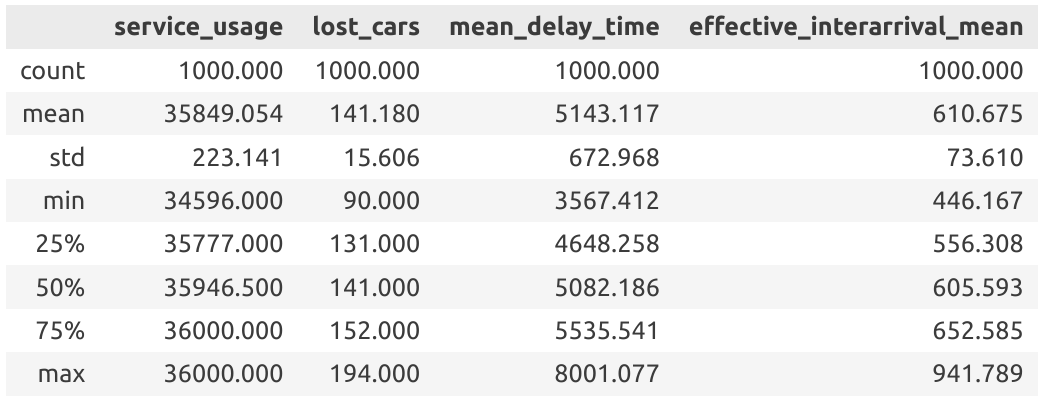
\includegraphics[width=0.8\textwidth]{./simple.png}
 \caption{\textbf{Sistema Original:}}
\end{figure}


\begin{figure}[htbp]
    \centering
    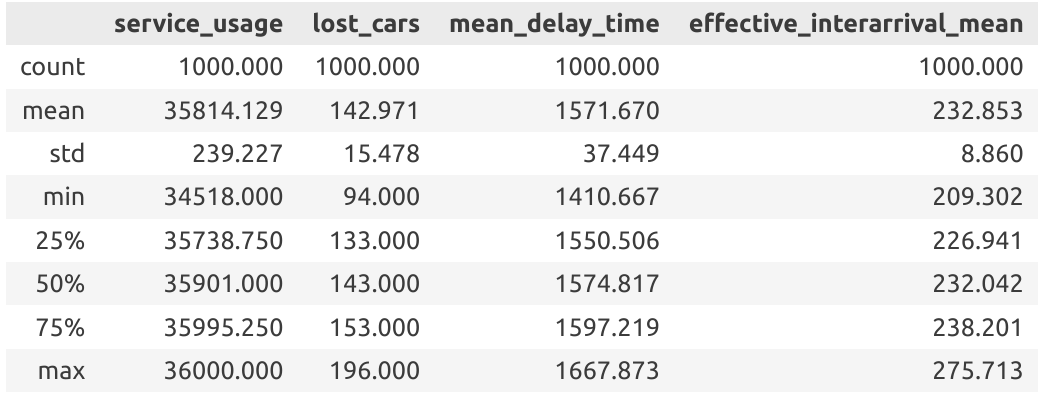
\includegraphics[width=0.8\textwidth]{./impatient.png}
   \caption{\textbf{Sistema Impaciente:}}
  \end{figure}

Como podemos observar, la cantidad de clientes perdidos al día y el tiempo de utilización del servidor en promedio son aproximadamente los mismos, mientras que para el sistema impaciente, se reducen en casi tres veces los tiempos de espera y los tiempos inter-arribos efectivos.

La explicación de este resultado, aparentemente contradictorio, está dada en que las pérdidas de clientes por impaciencias llevan a una reducción en las pérdidas por arribos al sistema lleno, manteniendo el total de clientes perdidos igual para ambos sistemas, y disminuyendo el tiempo inter-arribos efectivo. Además de esto, las salidas por impaciencia lleva a que los clientes que llegan a ser atendidos, pasen un tiempo menor en la cola (aquellos que pasan mucho se marchan de esta); esta última conclusión nos indica también, que si aumentáramos la media de la distribución normal truncada utilizada para modelar los tiempos de impaciencia, estos valores favorables para el sistema impaciente disminuirían.

\textbf{Dos servidores, una o dos colas (¿balanceadas?)}

De manera similar a la hipótesis anterior, los resultados obtenidos la refutaron; y es que las variables de interés obtuvieron valores casi idénticos para las tres simulaciones. Con lo que podemos afirmar que ninguna de los tres sistemas posee un mejor comportamiento.

\begin{figure}[htbp]
    \centering
    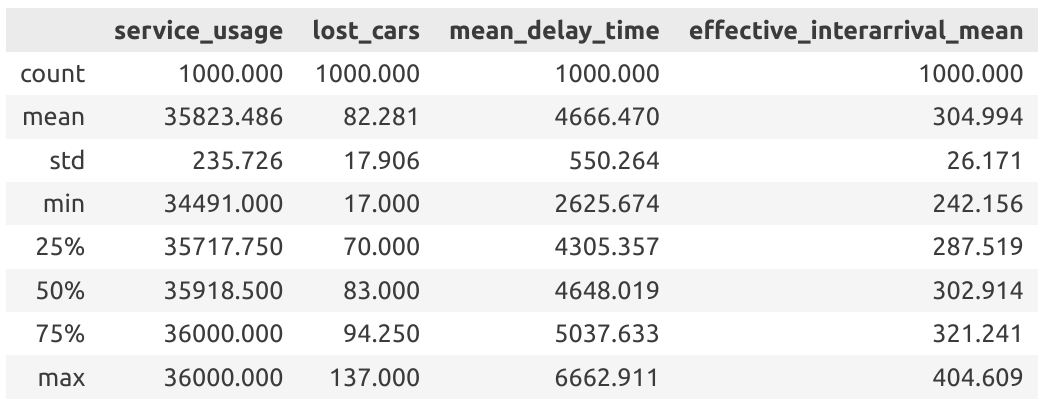
\includegraphics[width=0.8\textwidth]{./single_queue.png}
   \caption{\textbf{Single queue:}}
  \end{figure}

  \begin{figure}[htbp]
    \centering
    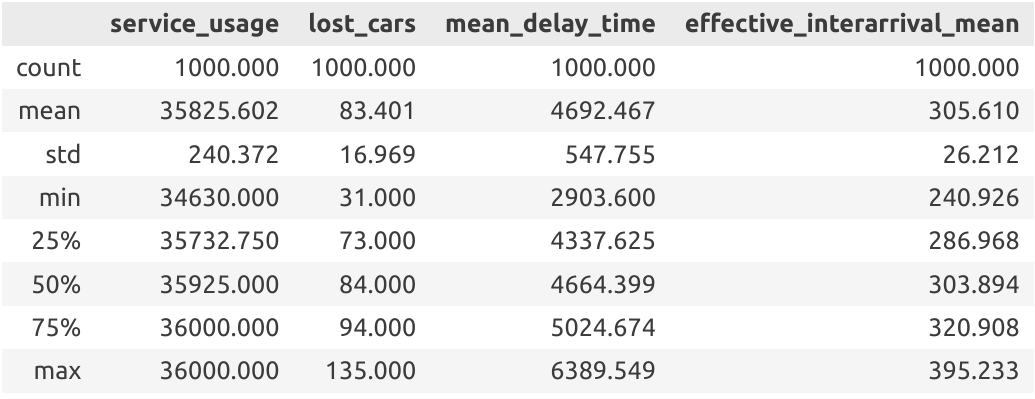
\includegraphics[width=0.8\textwidth]{./two_queues.png}
   \caption{\textbf{Two queues:}}
  \end{figure}

  \begin{figure}[htbp]
    \centering
    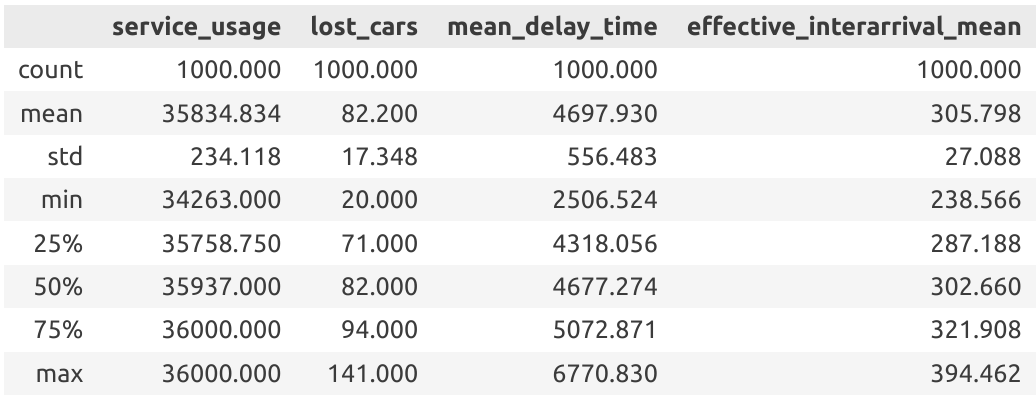
\includegraphics[width=0.8\textwidth]{./balanced_queues.png}
   \caption{\textbf{Balanced queues:}}
  \end{figure}


\subsection{Análisis de parada}

En el caso de las cadenas de Markov se realizaron las simulaciones un total de $200$ veces, dado que para realizar la simulación con tiempos de duración más grandes la complejidad computacional es suficiente como para que no sea posible realizar la simulación. La distribución de los clientes perdidos se puede observar en los histogramas anteriores mostrados. 

En el otro caso decidimos realizar las simulaciones un total de $1000$ veces, esta cantidad es computacional-mente posible y además como se puede ver en los siguientes gráficos las variables en cuestión tienden a seguir una distribución normal, (aunque en los test realizados no obtenemos eso).

\begin{figure}[htbp]
    \centering
    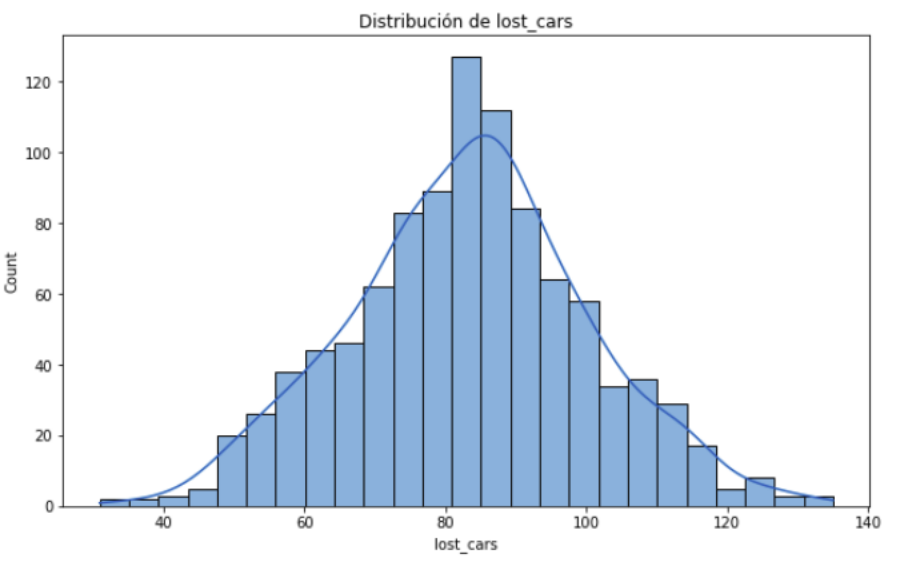
\includegraphics[width=0.6\textwidth]{./lost_carss.png}
  \end{figure}

  \begin{figure}[htbp]
    \centering
    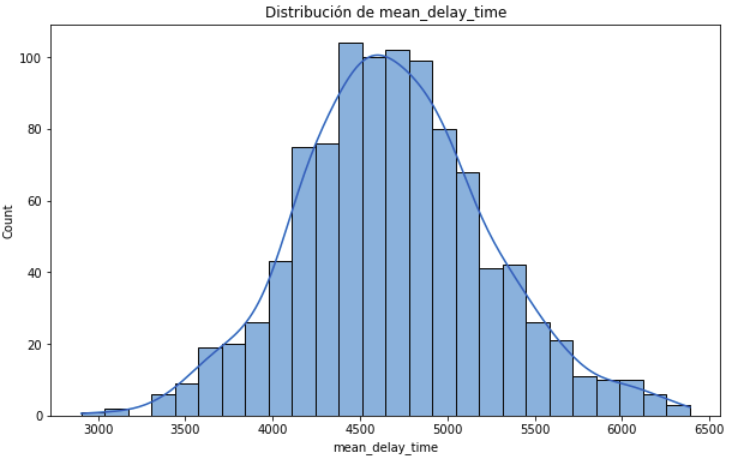
\includegraphics[width=0.6\textwidth]{./mean_delay_time.png}
  \end{figure}

  \begin{figure}[htbp]
    \centering
    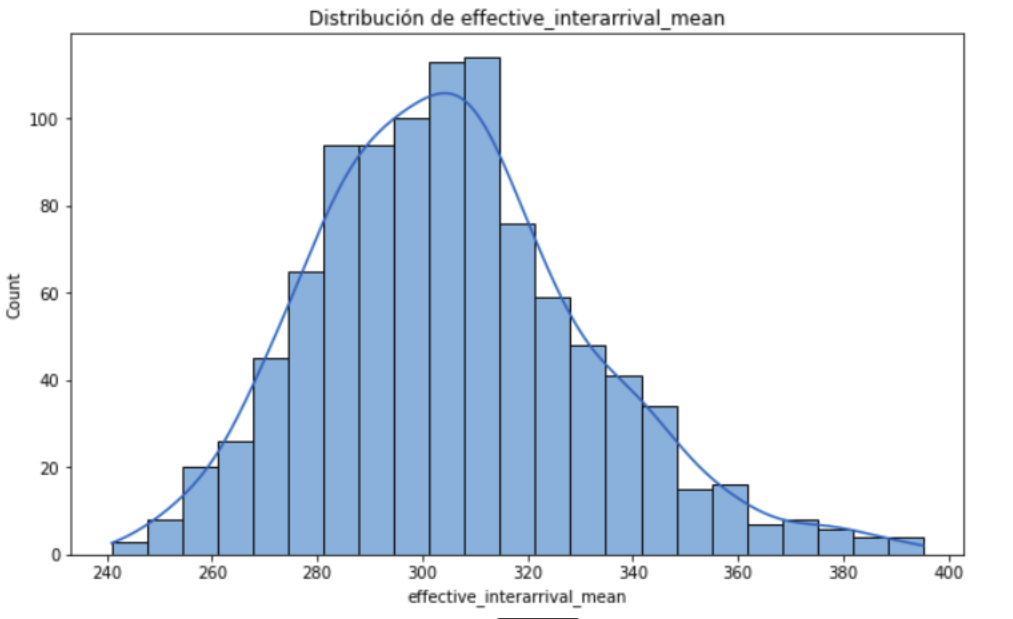
\includegraphics[width=0.6\textwidth]{./effective_interarrival_mean.png}
  \end{figure}

\end{document}